\lecture{2009-12-15}

Es gilt:
\begin{equation*}
	\cosh^2 x - \sinh^2 x = 1
\end{equation*}

\subsubsection*{Umkehrfunktionen}

\begin{equation*}
	\left.
	\begin{aligned}
		&\sinh x \text{ ist streng monoton } \leadsto \text{ umkehrbar} \\
		&\sinh x : \mathbb{R} \rightarrow \mathbb{R}
	\end{aligned}
	\right\} \arsinh x \text{ (Areasinus hyperbolicus)}
\end{equation*}

\paragraph{Explizite Angabe von $\arsinh x$}
\begin{align*}
	y &= \sinh x = \frac{\euler^x - \euler^{-x}}{2} \text{ Auflösen nach $x$}\\
	\implies 2y &= \euler^x - \euler^{-x} \quad| \cdot \euler^x \\
	\implies 2y \euler^x &= \euler^x \euler^x - \underbrace{\euler^x \euler^{-x}}_{=1} \\
	\implies \euler^{2x} - 2y\euler^x &= 1 \\
	\implies (\euler^x - y)^2 &= 1 + y^2 \\
	\implies \euler^x &= y + \sqrt{1 + y^2} \\
	\implies x &= \ln (y + \sqrt{1 + y^2}) = \arsinh x
\end{align*}

\paragraph{Folgerung}
\begin{multline*}
	\frac{\diff}{\diff x} \arsinh x = \frac{1}{x + \sqrt{1 + x^2}}\left(1 + \frac{1 \cdot 2x}{2\sqrt{1 + x^2}}\right) = \frac{1}{x + \sqrt{1 + x^2}} \left(1 + \frac{x}{\sqrt{1 + x^2}} \right) = \\
	= \frac{1}{x + \sqrt{1 + x^2}} \left(\frac{\sqrt{1 + x^2} + x}{\sqrt{1 + x^2}}\right) = \frac{1}{\sqrt{1 + x^2}}
\end{multline*}

\subsection{Fixpunkte, Iterationsverfahren}
Einer der ersten Schritte der Kurvendiskussion ist die Nullstellenbestimmung.

\subsubsection*{Nullstelle als Fixpunkt formulieren}

\begin{definition}
	$x^* \in [a, b]$ heißt Fixpunkt, falls gilt: $f: [a, b] \rightarrow \mathbb{R}: f(x^*) = x^*$
\end{definition}
\begin{lemma}
	Jeder Fixpunkt $x^*$ von $f$ ist Nullstelle der Funktion $g(x) = f(x) - x$. \\
	Umgekehrt: Jede Nullstelle von $f$ ist Fixpunkt von $g(x) = f(x) + x$.
\end{lemma}
\begin{definition}[Einstellige Fixpunktiteration]\flush
	\begin{equation*}
		x_{n + 1} = f(x_n) \qquad n \geq 0 \quad \text{zu gegebenem $x_0$}
	\end{equation*}
	(Im Folgenden sind alle Fixpunktiterationen einstellig.)
\end{definition}

\subsubsection*{Iterationsverläufe}
\begin{enumerate}
	\item $f(x) : 0 < f'(x) < 1$ (konvergente Iteration)
	\begin{center}
		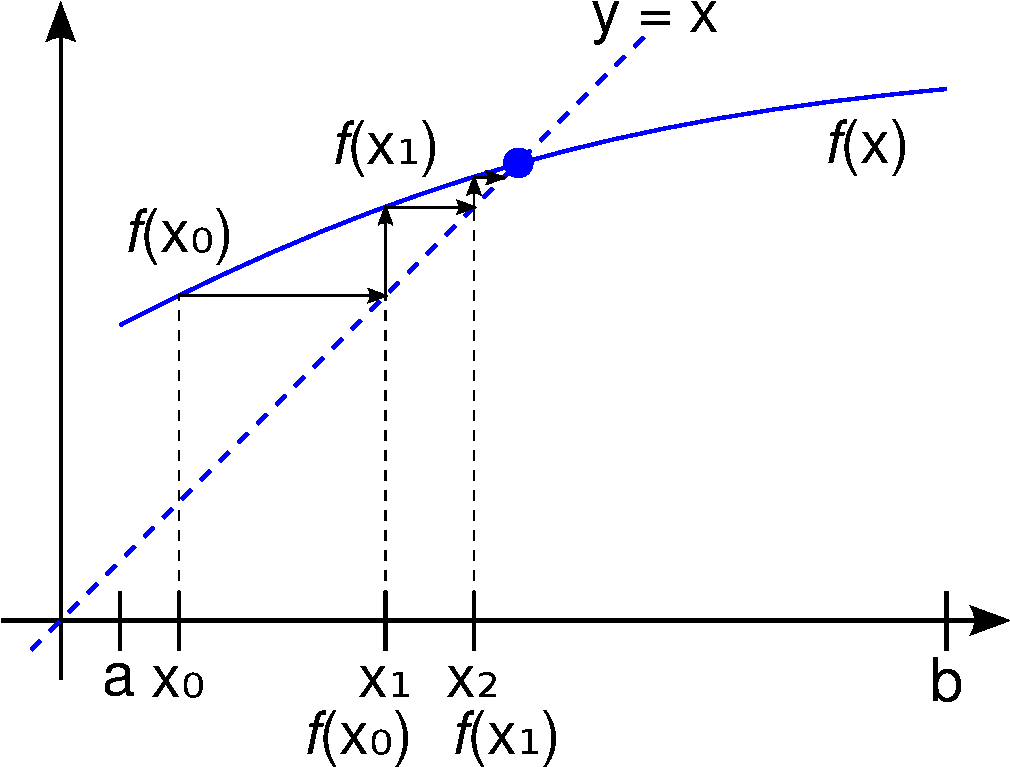
\includegraphics[width=0.4\textwidth]{include/20091215-1.pdf}
	\end{center}
	\item $f(x) : -1 < f'(x) < 0$ (konvergente Iteration)
	\begin{center}
		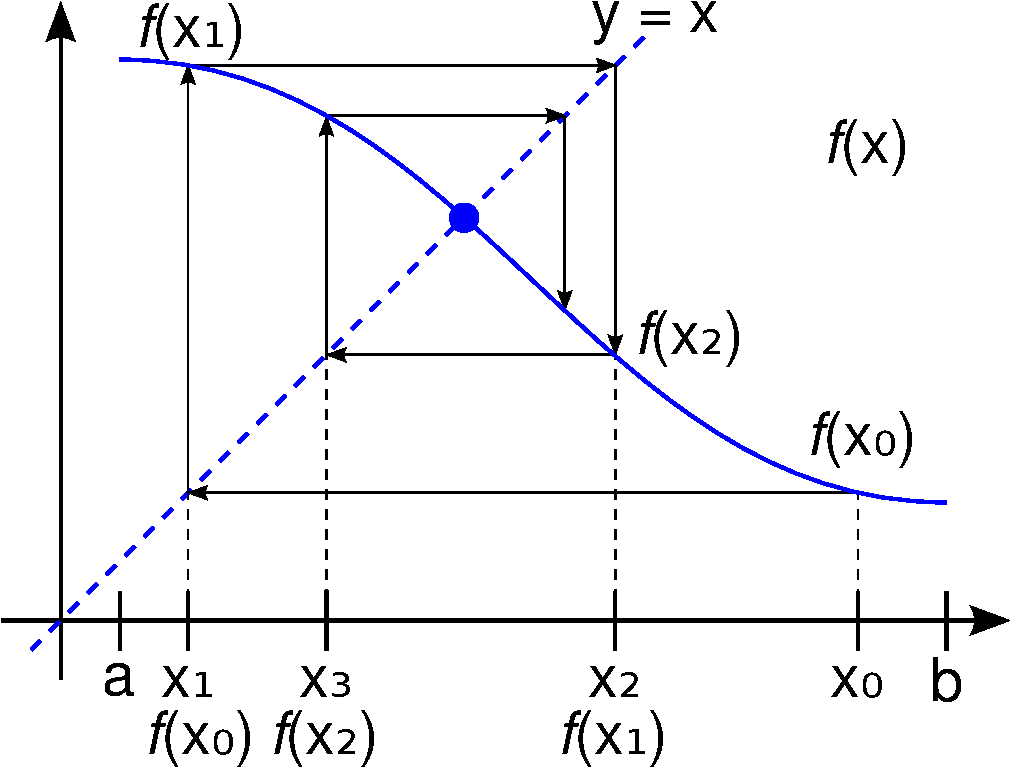
\includegraphics[width=0.4\textwidth]{include/20091215-2.pdf}
	\end{center}
	\item $f(x) : f'(x) > 1$ (divergente Iteration)
	\begin{center}
		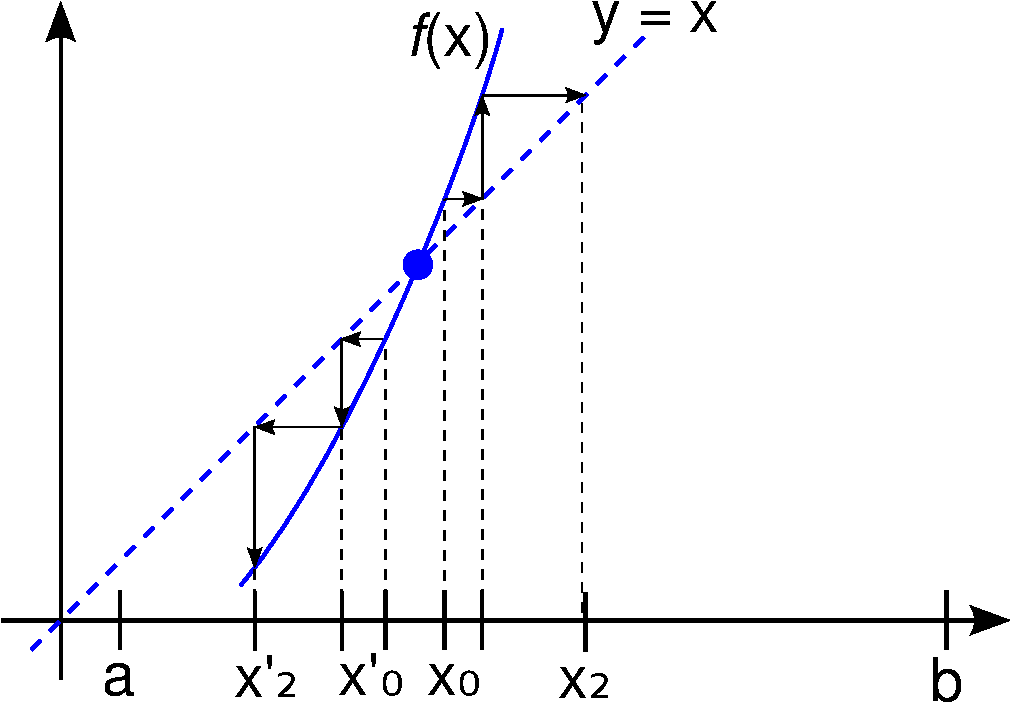
\includegraphics[width=0.4\textwidth]{include/20091215-3.pdf}
	\end{center}
\end{enumerate}

\begin{definition}[Lipschitz-Stetigkeit]
	Eine stetig differenzierbare Funktion $f: [a, b] \rightarrow \mathbb{R}$ heißt Lipschitz-stetig auf $[a, b]$, falls eine Lipschitz-Konstante $L$ existiert, mit
	\begin{equation*}
		|f(x_1) - f(x_2)| \leq L |x_1 - x_2| \qquad x_1, x_2 \in [a, b]
	\end{equation*}
	$f$ heißt \emph{kontrahierend}, falls $L < 1$.
\end{definition}
\begin{note}
	Aus dem 1. MWS folgt: $L = \underset{x \in ]a, b[}{\max} |f'(x)|$
\end{note}

\subsubsection*{Fixpunktsatz von Banach}
Wesentliche Voraussetzung: $f$ ist kontrahierend $\implies x_{n + 1} = f(x_n)$ ist konvergent
\begin{wrapfigure}[10]{r}{0.4\textwidth}
 	\centering
	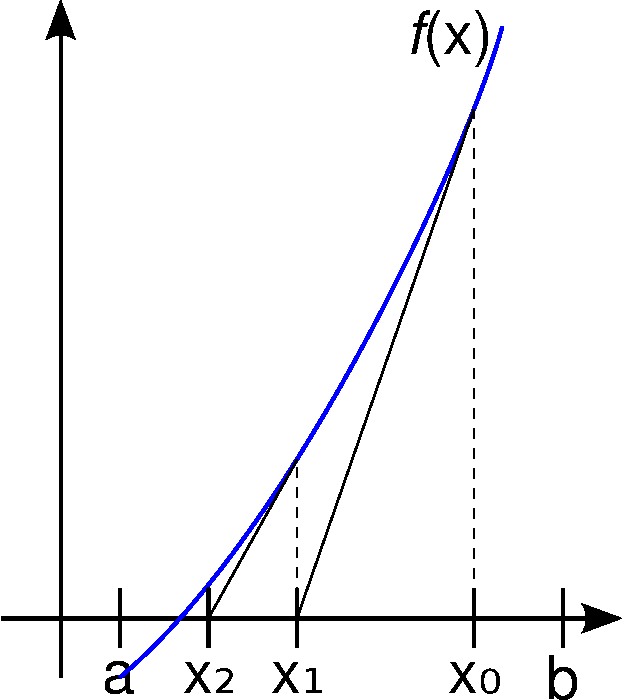
\includegraphics[width=0.4\textwidth]{include/20091215-4.pdf}
\end{wrapfigure}

\begin{note}
	Für nicht-kontrahierende Funktionen ist das Newton-Verfahren eine Abhilfe zur Nullstellensuche:
	\begin{align*}
		\text{Startwert}\:&:\: x_0 \\
		n \leq 0\:&:\:x_{n + 1} = x_n - \frac{f(x_n)}{f'(x_n)}
		\intertext{(Schnittgleichung: Tangente $\leftrightarrow$ x-Achse)}
	\end{align*}

	Das Newton-Verfahren ist (im Wesentlichen als einziges Verfahren) auf $\mathbb{R}^n$ verallgemeinerbar:
	\begin{align*}
		x_{n + 1} &= x_n + \Delta x_n \\
		\Diff f(x_n) \Delta x_n &= -f(x_n) \\
		\Delta x_n &= -\Diff f^{-1}(x_n) f(x_n)
	\end{align*}
\end{note}
